\chapter{Lecture 11 - More Complex Brayton Cycles}
\label{ch:ch11}
\section{Objectives}
The objectives of this lecture are:
\begin{enumerate}
\item Discuss impact of pressure ratio on cycle thermal efficiency
\item Regeneration and Regenerator effectiveness
\item intercooling and reheat
\end{enumerate}

\section{Pressure Ratio and Thermal Efficiency}
For an ideal cycle (isentropic compressor/turbine and no hydraulic losses) thermal efficiency is related to compressor pressure ratio as follows:
\begin{marginfigure}
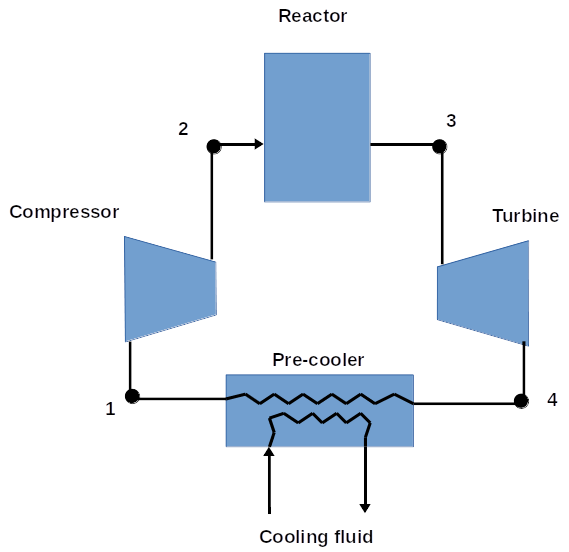
\includegraphics{simple_brayton.png}
\caption{Simple Ideal Brayton Cycle.}
\end{marginfigure}
\begin{align*}
\eta_{\text{TH}} &=\frac{w_{\text{net}}}{q_s} \\
                 &= \frac{C_p(T_3 - T_4) - C_p(T_2 - T_1)}{C_p(T_3 - T_2)} \\
                 &=\frac{(T_3 - T_2) - (T_4 - T_1)}{(T_3 - T_2)} \\
                 &=1 - \frac{T_4 - T_1}{T_3 - T_2} \\
                 &=1 - \frac{T_1(\sfrac{T_4}{T_1}-1)}{T_2(\sfrac{T_3}{T_2}-1)}
\end{align*}
If there are no pressure losses, then the pressure ratios for the compressor and turbine process are the same and $\sfrac{T_4}{T_1} = \sfrac{T_3}{T_2}$ so the last equality reduces to:
\begin{equation*}
\eta_{\text{TH}}=1 - \frac{T_1}{T_2}
\end{equation*}
Using our ideal gas relation for isentropic processes, $T_2 = T_1(r_p)^{\sfrac{(\gamma - 1)}{\gamma}}$ we obtain our final result in Equation \ref{eq:brayton_eff}.
\begin{equation}
\eta_{\text{TH}}=1 - \frac{1}{r_p^{\sfrac{(\gamma - 1)}{\gamma}}}
\label{eq:brayton_eff}
\end{equation}
For an ideal gas thermal efficiency increases for increasing pressure ratio. In principle this means we should be able to make thermal efficiency arbitrarily close to 100\% by increasing pressure ratio. In practice there are other considerations that need to be taken into account.

\section{Pressure Ratio and Net Specific Work}
\newthought{For many Brayton cycles} the pressure ratio affects achievable net specific work. This is because:
\begin{enumerate}
\item Real systems have limitations to the maximum temperature of the working fluid.  Some factors that lead to this limitation include:
\begin{enumerate}
\item material limits of the system piping and structural components
\item material limits of the heat source---such as nuclear reactor core outlet temperature limits---which, in order to add heat to the working fluid, are an upper bound to the maximum Brayton cycle system temperature.
\end{enumerate}
As pressure ratio increases, so does the temperature at the compressor discharge ($T_2$), so these maximum temperature limits impose a limit to the compressor pressure ratio.  Advances in material sciences offer the possibility of increasing these temperature limits over time but, for any concept, the designer has limited ability to influence this bound.
\item Real systems have limits to the minimum temperature of the working fluid.  This is dictated by the temperature of the thermal reservoir to which the cycle must reject heat in the pre-cooler.  This environmental temperature is generally outside of the control of the designer.  
\end{enumerate}
 
\begin{marginfigure}
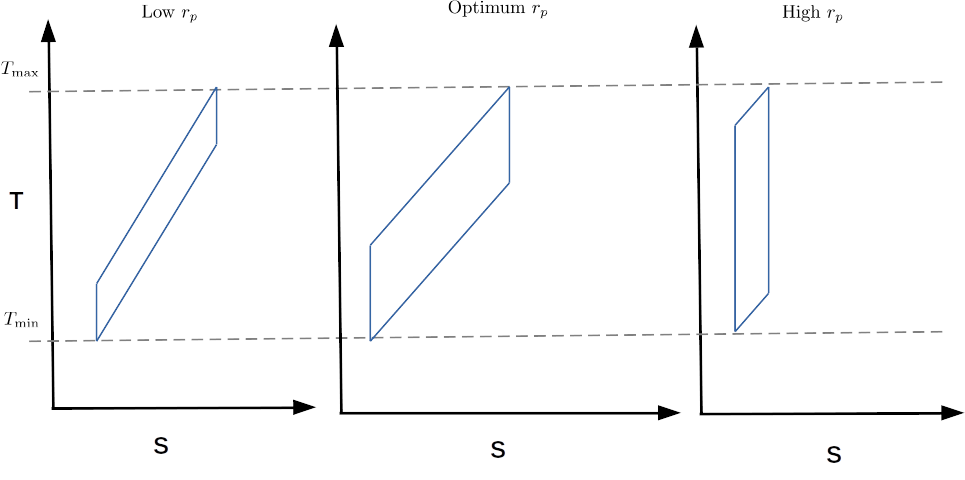
\includegraphics{brayton_wnet_vs_rp.png}
\caption{Effect of $r_p$ on $w_{\text{net}}$ for simple ideal Brayton cycles.}
\label{fig:wnet_vs_rp}
\end{marginfigure}
\newthought{These limits influence} the maximum net specific work that can be extracted from the working fluid for an ideal Brayton cycle. Figure \ref{fig:wnet_vs_rp} gives a qualitative feel for the influence of pressure ratio on net specific work for systems operating within material limits. Some key points:
\begin{itemize}
\item At low $r_p$, most of the added heat is simply rejected to the environment. 
\item At high $r_p$, the amount of heat that can be added to the working fluid is constrained by the temperature limit; thermal efficiency is high but, since $w_{\text{net}}$ is limited, the mass flow rate of the coolant must be higher to achieve a desired power output.
\item The optimum $r_p$ is a function of the working fluid. Figure \ref{fig:wnet_vs_rp_fluid} illustrates this for four typical Brayton cycle working fluids. 
\end{itemize}

\begin{marginfigure}
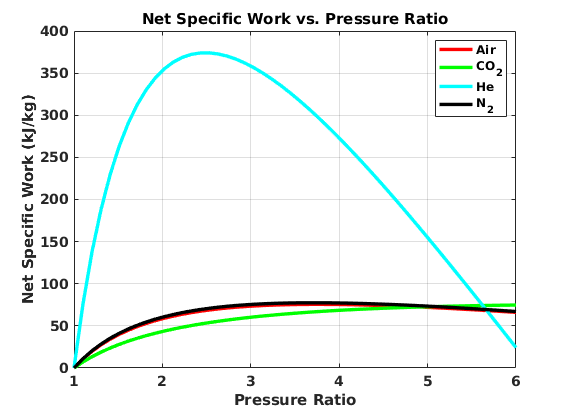
\includegraphics{Brayton_wnet_vs_rp_and_fluid.png}
\caption{Net specific work vs pressure ratio for common fluids.}
\label{fig:wnet_vs_rp_fluid}
\end{marginfigure}

\marginnote[0.5cm]{\textbf{Note:} looking at Figure \ref{fig:wnet_vs_rp_fluid}, which fluid is different from the others?}

\begin{itemize}
\item Reduced $w_{\text{net}}$ and increased $\dot{m}$ of working fluid may seem like a small price to pay for increased thermal efficiency but:
\begin{itemize}
\item Real systems will suffer hydraulic pressure losses that are proportional to $\dot{m}$
\item The thermal efficiency of a Brayton cycle is heavily impacted by those hydraulic pressure losses as we will see from our exercises.
\item Sadly a detailed treatment which connects all of the dots between pressure ratio, working fluid mass flow rate, and analysis of thermal efficiency including hydraulic pressure losses still needs to be brought into the scope of this class.
\end{itemize} 

\end{itemize}

\index{Brayton cycle, regeneration}
\section{Brayton Cycle with Regeneration}

\begin{marginfigure}
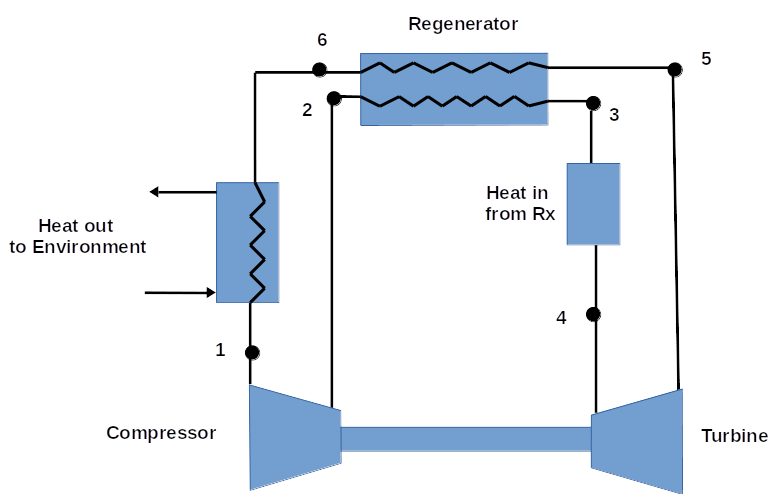
\includegraphics{brayton_regen.png}
\caption{Schematic of a regenerative Brayton cycle.}
\label{fig:brayton_regen}
\end{marginfigure}
\begin{marginfigure}
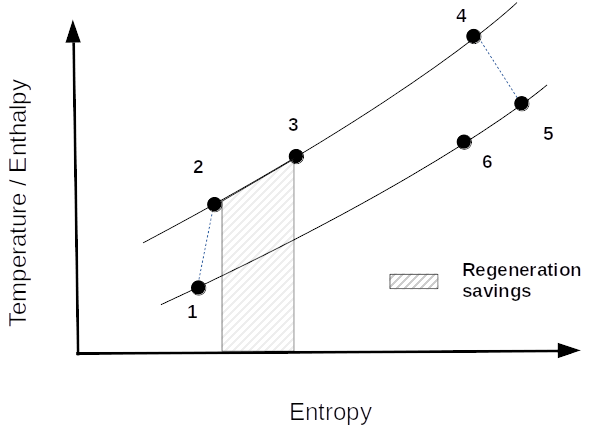
\includegraphics{brayton_regen_TS.png}
\caption{Reduced $q_s$ due to regeneration savings}
\label{fig:brayton_regen_TS}
\end{marginfigure}

\newthought{One obvious weakness} of the simple ideal Brayton cycle is the large amount of useful energy that gets rejected to the environment.  The working fluid at the turbine exhaust (state point 4) is at low pressure but its temperature remains high.  We can exploit the exergy contained in this high temperature fluid in a regenerator as illustrated in Figure \ref{fig:brayton_regen}.  Use of the regenerator reduces the amount of energy that need be added in the heat addition process.  This is illustrated in Figure \ref{fig:brayton_regen_TS}.



\index{regenerator effectiveness}
\newthought{We characterize the performance} of the regenerator with a parameter called \emph{regenerator effectiveness}.\marginnote[0.25cm]{\textbf{regenerator effectiveness:} the ratio of the actual enthalpy increase of the fluid on the low temperature side to the maximum theoretical enthalpy increase.}  The regenerator effectiveness for this cycle can be expressed as in Equation \ref{eq:regen_eff}.
\begin{equation}
\eta_{\text{reg}} = \frac{\Delta h_{\text{actual}}}{\Delta h_{\text{max}}} = \frac{h_3 - h_2}{h_5 - h_2}
\label{eq:regen_eff}
\end{equation}
Having a higher regenerator effectiveness is obviously desirable but is subject to limits.  Qualitatively speaking one increases regenerator effectiveness by:
\begin{itemize}
\item Increasing heat transfer surface area in the regenerator---e.g. make the regenerator bigger.
\item Enhancing heat transfer effectiveness in the regenerator. This might be done by:
\begin{itemize}
\item use materials with better conductive heat transfer properties
\item use convective heat transfer enhancements such as spiral grooves.  
\end{itemize}
\item use working fluids with better heat transfer properties.
\end{itemize}
With the exception of convective heat transfer enhancements which we will discuss in a later lecture, these considerations are beyond the scope of this course. Like isentropic efficiency data for pumps, compressors, and turbines, we will take regenerator effectiveness to be a given parameter.  \textbf{A typical value will be around 60\%.}

\section{Inter-cooling} \index{Brayton cycle, inter-cooling}
\begin{marginfigure}
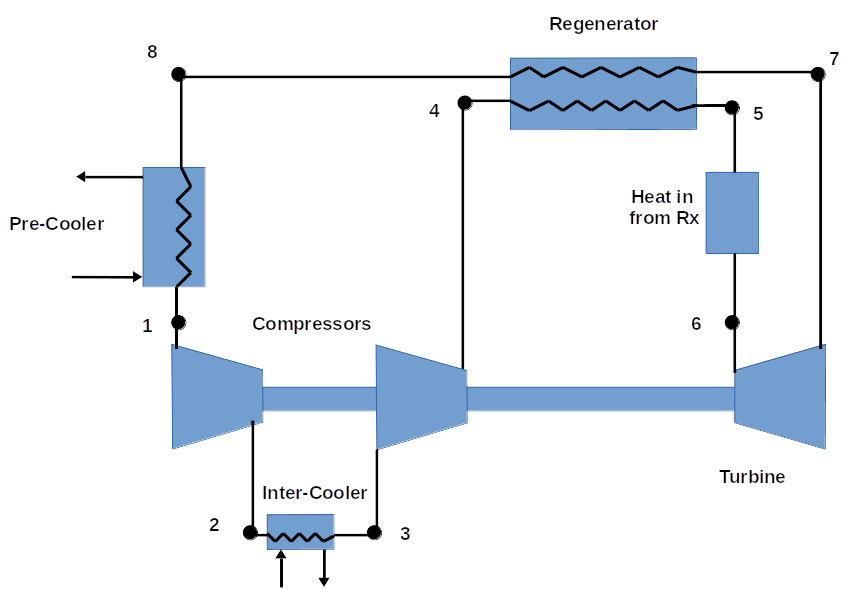
\includegraphics{brayton_regen_IC.png}
\caption{Brayton cycle with regeneration and intercooling.}
\label{fig:brayton_regen_IC}
\end{marginfigure}

\begin{marginfigure}
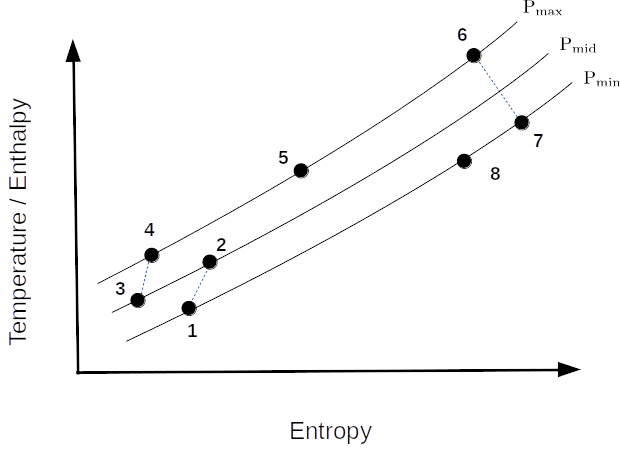
\includegraphics{brayton_IC_TS.png}
\caption{TS plot of a Brayton cycle with regeneration and inter-cooling.}
\label{fig:brayton_IC_TS}
\end{marginfigure}

\begin{marginfigure}
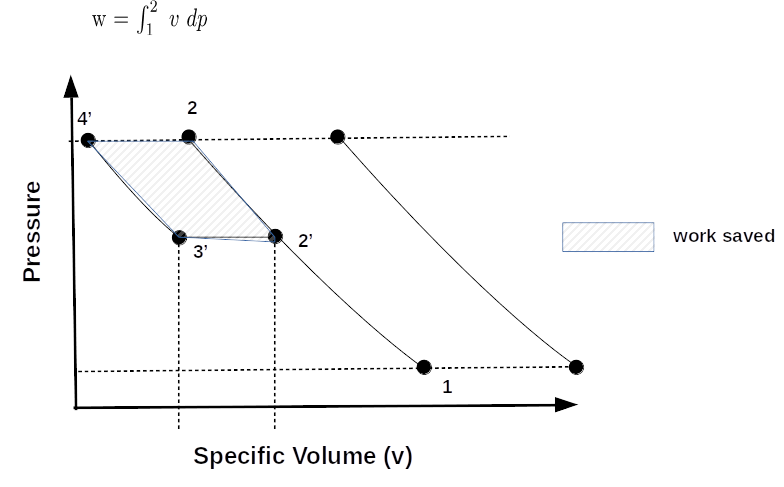
\includegraphics{brayton_IC_pv.png}
\caption{Work savings from inter-cooling.}
\label{fig:brayton_IC_pv}
\end{marginfigure}
\newthought{In addition to} using regeneration to reduce heat rejected, it is desirable to reduce the work required in the compression processes.  As characterized by the back work ratio, as much as half (or more!) of the turbine work for a Brayton cycle may be needed to power the compressor.  We can reduce the work required for compression by \emph{cooling} the working fluid part-way through the compression.  A Brayton cycle schematic with such an \emph{inter-cooler} is shown in Figure \ref{fig:brayton_regen_IC}. Heat extracted in the inter-cooler is normally rejected to the environment.  In this sense the energy is lost but the savings on compressor work more than offsets this sacrifice.  While it's traditional to show the temperature-entropy diagram---this is shown in Figure \ref{fig:brayton_IC_TS}---the work savings from inter-cooling is more easily seen from the $P-v$ diagram in Figure \ref{fig:brayton_IC_pv}. 



\newthought{A natural question} to ask is: How much of the compression should be done with the first compressor and how much with the second to get maximum work reduction?  It is a straight-forward but tedious task to show that, for isentropically ideal compressors, you \emph{minimize overall compressor work if the pressure ratios for the compressors are the same.}  

\index{Brayton cycle, reheat}

\section{Brayton Cycle with Reheat}


\newthought{Another way to increase} the net specific work and thermal efficiency of a Brayton cycle is to include one or more stages of reheat.  A T-S diagram is shown in Figure \ref{fig:brayton_IC_RH_TS} and a schematic representation of such a cycle is illustrated in Figure \ref{fig:brayton_IC_RH}.
\begin{marginfigure}
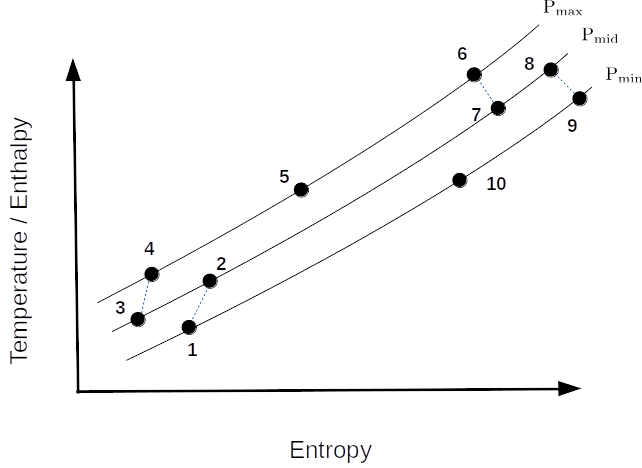
\includegraphics{brayton_IC_RH_TS.png}
\caption{T-S diagram for Brayton cycle with reheat.}
\label{fig:brayton_IC_RH_TS}
\end{marginfigure}

\begin{figure}
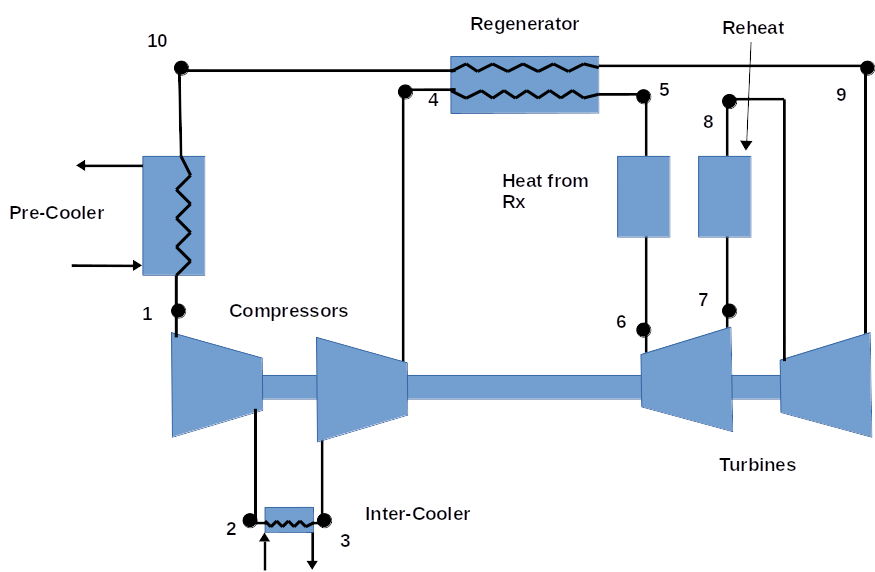
\includegraphics{brayton_IC_RH.png}
\caption{Brayton cycle with reheat.}
\label{fig:brayton_IC_RH}
\end{figure}

You should be asking the same question as with intercooling: how do I set the pressure ratios for the turbines such that I get maximum benefit from reheating?  Sadly I do not have a short answer to this question. To help you build some intuition on this, we will investigate this issue in our workshop assignments.


